\section{Preprocessing}
\subsection{3D to 2D conversion}
\nblink{brats/02\_preprocess.ipynb}
The scans in the BraTS datasets are 3D volumes. There is no general limitation of neural networks to work with 3D input, but 3D volumes are very big and would require many input neurons which in turn increases the model size and training time significantly.

We therefore decided to extract three horizontal slices from the 3D volume and save them as normal gray-scale images.
The extracted slice should show a part of the tumor in the brain, hence we can not just take random slices from a volume.

The used algorithm works like this (see Figure \ref{preprocessing_layers} for a graphical explanation):

\begin{itemize}
    \item From the top of the brain, search downwards on all modalities until the top of the tumor is found
    \item From the bottom of the brain, search upwards on all modalities until the bottom of the tumor is found
    \item Take the first slice 25\% into the tumor from the top to the bottom
    \item Take the second slice in the middle of the top and bottom of the tumor
    \item Take the last slice 25\% into the tumor from the bottom to the top
\end{itemize}

\begin{figure}[H]
    \centering
    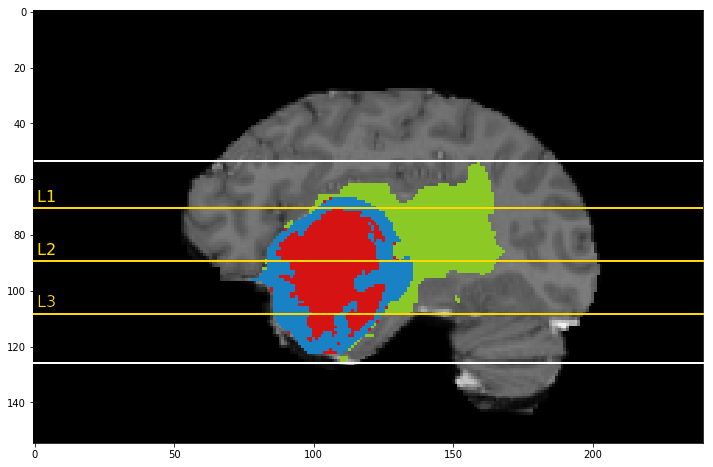
\includegraphics[width=14cm]{chapters/04_segmentation/images/slicing.png}
    \caption{Extracting three 2D layers from the 3D volume. Search top and bottom of the tumor (white lines). Extract layer L1 at 25\% from the top to bottom, L2 at 50\% and L3 at 75\%.}
    \label{preprocessing_layers}
\end{figure}


\subsection{Training and test data split}
\nblink{brats/03\_train\_test\_split.ipynb}

Slices taken from the same brain look very similar. It would be very easy for a neural network to correctly segment an image when an image from the same brain was part of the training data set.
We therefore split up the preprocessed dataset into a training and a test set while keeping the slices from the same brain in the same set.
